% Problem 6/2 solution
\noindent
\underline{Solution:}\\

\begin{enumerate}
\item In $^1D_2$ state there are no unpaired electrons (singlet state) and hence the total spin $S = 0$. The angular momentum quantum number $L = 2$, which means that the total angular momentum $\left<\vec{\hat{L}}^2\right> = 2(2 + 1)\hbar^2 = 6\hbar^2$. The total angular momentum quantum number $J = 2$ (specified by the subscript). In $^3F_4$ state the multiplicity ($2S+1$) is 3 which gives $S = 1$ (triplet state) and $F$ term implies $L = 3$. The total angular momentum quantum number is specified as $J = 4$.
\item The energy level diagram for alkai metal atoms is:

\begin{figure}[htp!]
\centering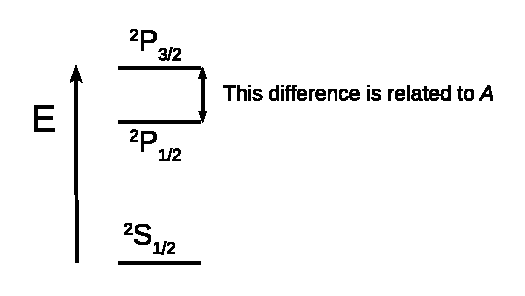
\includegraphics[scale=0.7]{diagram}
\end{figure}

The two emission lines originate from the two $^2P$ states, which are split by the spin-orbit interaction, and terminate to the ground $^2S$ state.
Hence the energy difference between the two emission lines gives the energy difference between the spin-orbit split states $^2P_{1/2}$ and $^2P_{3/2}$.
The line positions must be converted to energy by relation $E = h\nu = \frac{hc}{\lambda}$ ($h$ is the Planck's constant and $c$ is the speed of light).
To calculate $A$, we have to calculate the energy difference between $^2P_{1/2}$ and $^2P_{3/2}$:
\begin{eqnarray}
\nonumber
& & ^2P_{1/2}\textnormal{: }E_{SO} = \frac{A}{2}\left[J(J+1) - L(L+1) - S(S+1)\right] = -A\\
\nonumber
& & ^2P_{3/2}\textnormal{: }E_{SO} = \frac{A}{2}\left[J(J+1) - L(L+1) - S(S+1)\right] = \frac{1}{2}A\\
\nonumber
& & \Delta E_{SO} = \frac{3}{2}A
\end{eqnarray}

Next we calculate the energies for the observed transitions. For $^2P_{3/2}\rightarrow ^2S_{1/2}$ we have:
\begin{eqnarray}
\nonumber
& & E_1 = h\nu_1 = hc / \lambda_1 = (6.6261\times 10^{-34}\textnormal{ Js})\times\frac{2.9979\times 10^8\textnormal{m/s}}{766.70\times 10^{-9}\textnormal{ m}}\\
\nonumber
& &  = 2.5909\times 10^{-19}\textnormal{ J} = 1.6171\textnormal{ eV} = 13043\textnormal{ cm}^{-1}
\end{eqnarray}

For $^2P_{1/2}\rightarrow ^2S_{1/2}$:

\begin{eqnarray}
\nonumber
& & E_2 = h\nu_2 = hc / \lambda_2 = (6.6261\times 10^{-34}\textnormal{ Js})\times\frac{2.9979\times 10^8\textnormal{m/s}}{770.11\times 10^{-9}\textnormal{ m}}\\
\nonumber
& &  = 2.5794\times 10^{-19}\textnormal{ J} = 1.6099\textnormal{ eV} = 12985\textnormal{ cm}^{-1}
\end{eqnarray}

Thus the energy difference is $\Delta E_{SO} = 39$ cm$^{-1}$ which gives $A = 2\Delta E_{SO} / 3 = 39$ cm$^{-1}$.

\item The selection rule is $\Delta l = \pm 1$. For $5d\rightarrow 2s$ we have $\Delta l = -2$ and hence it is forbidden. Transition $5p\rightarrow 3s$ has $\Delta l = -1$ and therefore it is allowed. $5p\rightarrow 3f$ has $\Delta l = +2$ and it is forbidden.

\end{enumerate}

\hrule\vspace{0.5cm}
